%%%%%%%%%%%%%%%%%%%%%%%%%%%%%%%%%%%%%%%%%%%%%%%%%%%%%%%%%%%%%%%%%%%%%%%%%%%%%%%%%%
\begin{frame}[fragile]\frametitle{}
\begin{center}
{\Large Conclusions}
\end{center}
\end{frame}

%%%%%%%%%%%%%%%%%%%%%%%%%%%%%%%%%%%%%%%%%%%%%%%%%%%%%%%%%%%%%%%%%%%%%%%%%%%%%%%%%%
\begin{frame}[fragile]\frametitle{How to Build an AI Agent?}

	\begin{center}
	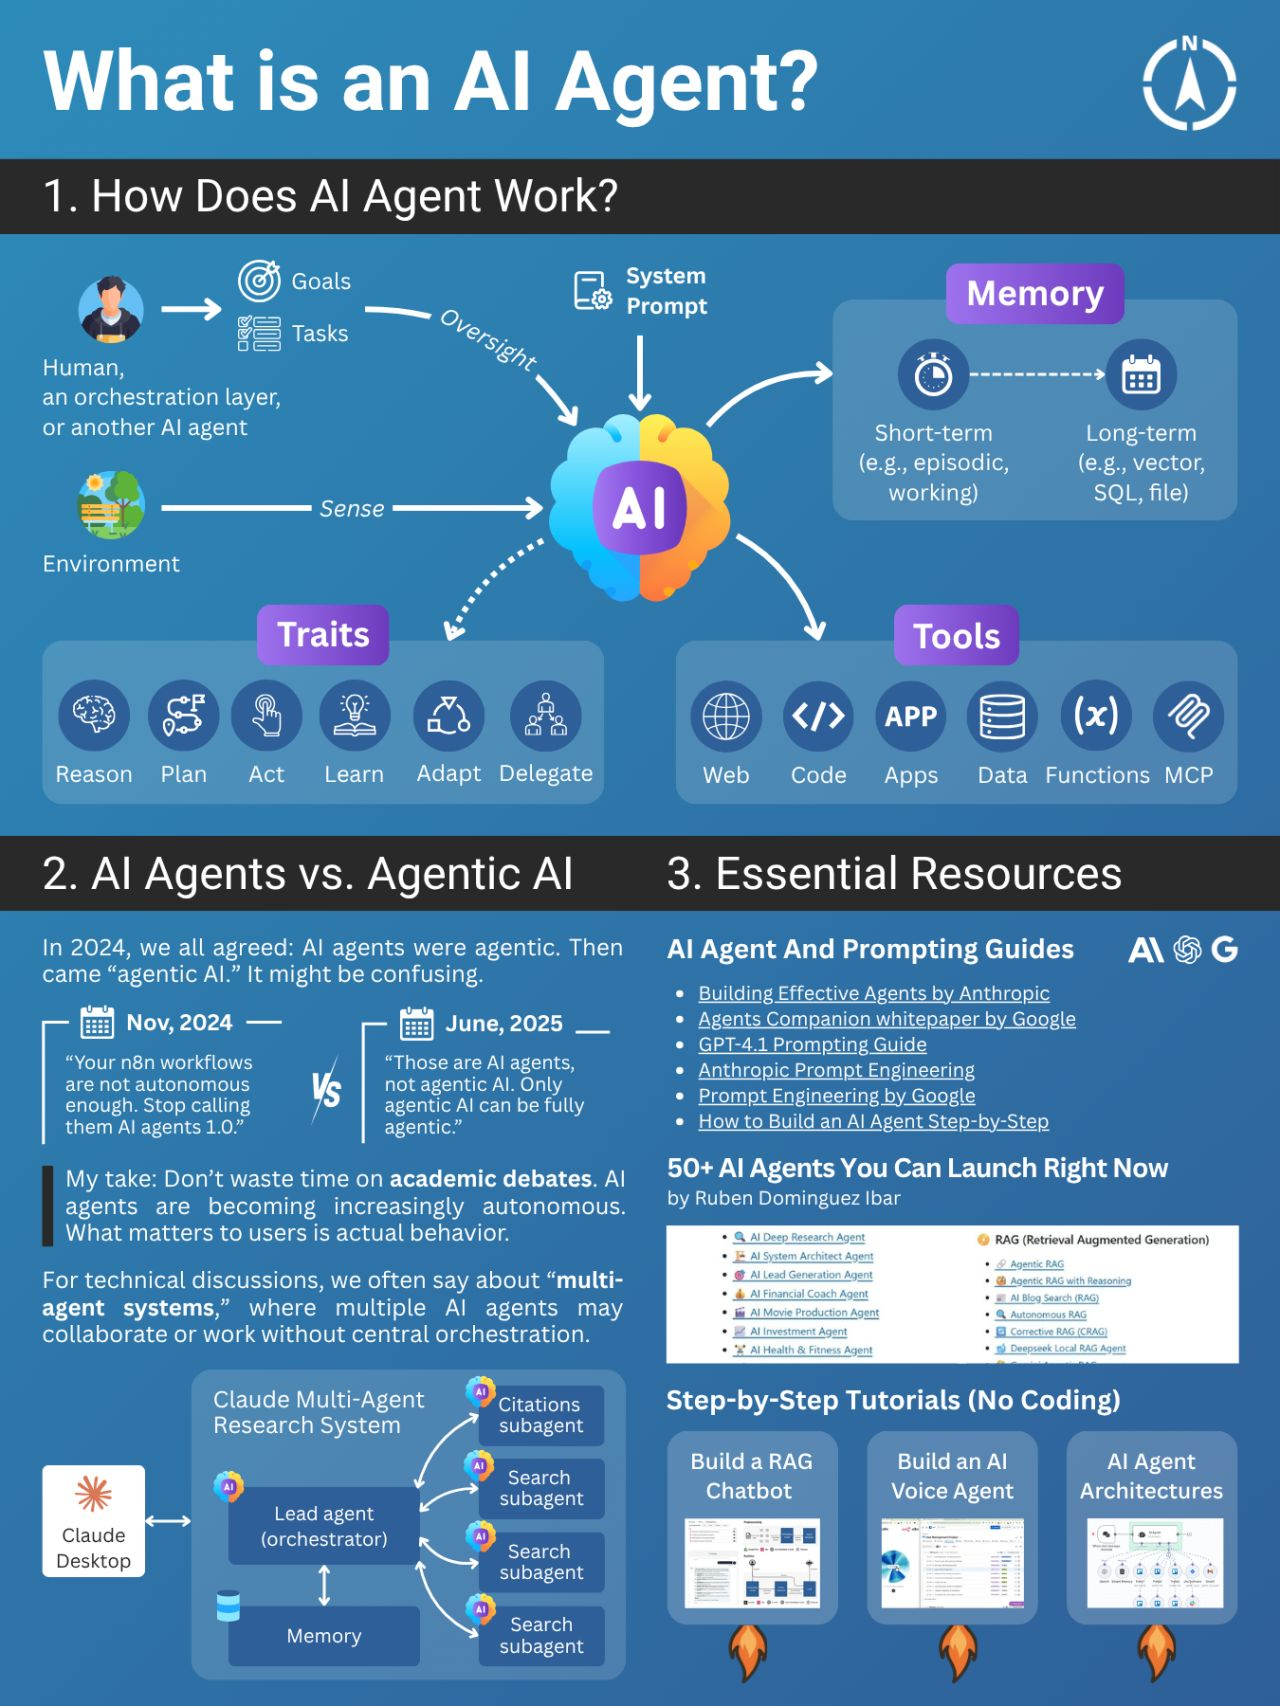
\includegraphics[width=0.45\linewidth,keepaspectratio]{aiagents8}
	
	{\tiny (Ref: LinkedIn post by Pawl Huryn)}
	
	\end{center}
	
\end{frame}


%%%%%%%%%%%%%%%%%%%%%%%%%%%%%%%%%%%%%%%%%%%%%%%%%%%%%%%%%%%
\begin{frame}[fragile]\frametitle{What’s Still Hard: Observability}

      \begin{itemize}
        \item Observability tracks agent behavior at each step
        \item Essential: logs of tool calls, retries, decisions
        \item Use metrics to catch latency and cost issues
        \item Debug via step-wise traceability
        \item Detect when agents go off-rail
        \item Tools like Comet Opik support observability
        \item Must be designed in from day one
        \item Critical for high-autonomy agent systems
      \end{itemize}

\end{frame}

%%%%%%%%%%%%%%%%%%%%%%%%%%%%%%%%%%%%%%%%%%%%%%%%%%%%%%%%%%%
\begin{frame}[fragile]\frametitle{What’s Still Hard: Evaluation}

      \begin{itemize}
        \item Agents are non-deterministic — need ongoing evaluation
        \item Track goal/task success rates regularly
        \item Monitor tool call success and failure
        \item Measure RAG quality and hallucination rate
        \item Check for overthinking or inefficiency
        \item Analyze latency and token usage per step
        \item Avoid "vibe checks"; use real metrics
        \item Evaluation is agentic system QA
      \end{itemize}

\end{frame}

%%%%%%%%%%%%%%%%%%%%%%%%%%%%%%%%%%%%%%%%%%%%%%%%%%%%%%%%%%%
\begin{frame}[fragile]\frametitle{Agentic AI: Protocols > Prompts}
\begin{columns}
    \begin{column}[T]{0.6\linewidth}
      \begin{itemize}
        \item Handcrafted prompts won't scale with system complexity
        \item Shift toward shared protocols and standards
        \item MCP: standardizes structured context inputs
        \item Includes tools, memory, RAG, prior instructions
        \item A2A by Google: enables agent-to-agent messaging
        \item Shared schemas will aid cross-agent collaboration
        \item Protocols bring cleaner, reusable abstractions
        \item Adoption may take time, like HTTP in the past
      \end{itemize}
    \end{column}
    \begin{column}[T]{0.4\linewidth}
        \begin{center}
        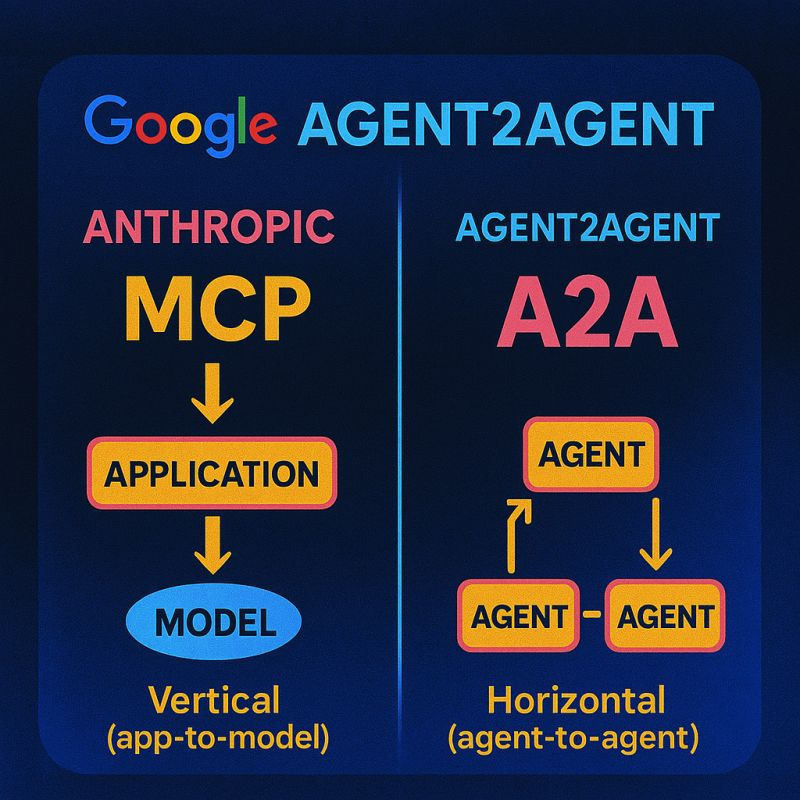
\includegraphics[width=0.8\linewidth,keepaspectratio]{aiagents24}
		
		{\tiny (Ref: LinkedIn post by Reuven COhen)}
        \end{center}	
    \end{column}
\end{columns}
\end{frame}

%%%%%%%%%%%%%%%%%%%%%%%%%%%%%%%%%%%%%%%%%%%%%%%%%%%%%%%%%%%
\begin{frame}[fragile]\frametitle{Agentic AI: Hybrid Reasoning Models}

      \begin{itemize}
        \item Future agents will combine planning and fast actions
        \item One model can't do everything efficiently
        \item Use reasoning when needed, act quickly otherwise
        \item Models like Claude 3.7 are early examples
        \item Hybrid approaches balance intelligence and speed
        \item Reduces unnecessary overthinking by agents
        \item Improves responsiveness and resource use
      \end{itemize}
\end{frame}

%%%%%%%%%%%%%%%%%%%%%%%%%%%%%%%%%%%%%%%%%%%%%%%%%%%%%%%%%%%
\begin{frame}[fragile]\frametitle{Agentic AI: Better Memory Systems}

      \begin{itemize}
        \item Memory is currently poorly integrated
        \item Future: smarter, context-aware memory systems
        \item Recall what matters — when and why
        \item Memory scoped to tasks, sessions, or personas
        \item Easier to manage and debug
        \item Improves relevance and performance of agents
        \item Critical for long-term agent autonomy
      \end{itemize}

\end{frame}

%%%%%%%%%%%%%%%%%%%%%%%%%%%%%%%%%%%%%%%%%%%%%%%%%%%%%%%%%%%
\begin{frame}[fragile]\frametitle{Agentic AI: Tool Ecosystem Maturity}

      \begin{itemize}
        \item Current tools are often custom and ad hoc
        \item Maturing ecosystem will offer plug-and-play APIs
        \item Expect reusable, trusted tool interfaces
        \item Better abstraction layers will emerge
        \item Shared security and usage practices will develop
        \item Inspired by microservice evolution in software
        \item Enables scalable and secure agent systems
      \end{itemize}

\end{frame}




%%%%%%%%%%%%%%%%%%%%%%%%%%%%%%%%%%%%%%%%%%%%%%%%%%%%%%%%%%%%%%%%%%%%%%%%%%%%%%%%%%
\begin{frame}[fragile]\frametitle{Key Principles for LLM Success}
    \begin{itemize}
        \item Focus on building the right system, not the most sophisticated one
        \item Progress systematically:
            \begin{itemize}
                \item Start with simple prompts
                \item Optimize through comprehensive evaluation
                \item Add multi-step agents only when necessary
            \end{itemize}
        \item Core implementation principles:
            \begin{itemize}
                \item Maintain simplicity in agent design
                \item Ensure transparency in planning steps
                \item Carefully design agent-computer interface (ACI)
            \end{itemize}
        \item Consider reducing framework abstraction layers in production
        \item Goal: Create powerful, reliable, and maintainable agents
    \end{itemize}
\end{frame}

%%%%%%%%%%%%%%%%%%%%%%%%%%%%%%%%%%%%%%%%%%%%%%%%%%%%%%%%%%%
\begin{frame}[fragile]\frametitle{In General}
  \begin{itemize}
    \item Autonomous AI Agents powered by Large Language Models represent AI pinnacle.
    \item Abilities in planning, memory utilization, and tool use, combined with a flawless workflow, open exciting possibilities across industries.
    \item A future where AI-driven efficiency and problem-solving reach unprecedented heights.
    \item Machines that think, remember, and adapt - a revolution in AI.
  \end{itemize}
\end{frame}


%%%%%%%%%%%%%%%%%%%%%%%%%%%%%%%%%%%%%%%%%%%%%%%%%%%%%%%%%%%%%%%%%%%%%%%%%%%%%%%%%%
\begin{frame}[fragile]\frametitle{Challenges in LLM-Centered Agents}
  \begin{itemize}

    \item Finite Context Length: Restricted context capacity limits inclusion of historical information, detailed instructions, API call context, and responses.
    % \item System design works with limited communication bandwidth, impacting mechanisms like self-reflection.
    \item Long-term planning and task decomposition: LLMs struggle to adjust plans when faced with unexpected errors.
    % \item Planning over lengthy history and exploring solution space remain challenging for LLMs.
    \item Less robust compared to humans who learn from trial and error.
    % \item Reliability of Natural Language Interface: Current agent system relies on natural language as an interface, but the reliability of model outputs is questionable.
    \item LLMs may make formatting errors and occasionally exhibit rebellious behavior (e.g., refuse to follow an instruction).
    % \item Agent demo code often focuses on parsing model output due to these reliability issues.
  \end{itemize}
\end{frame}

%%%%%%%%%%%%%%%%%%%%%%%%%%%%%%%%%%%%%%%%%%%%%%%%%%%%%%%%%%%%%%%%%%%%%%%%%%%%%%%%%%
\begin{frame}[fragile]\frametitle{When to Use Agents}
\begin{itemize}
    \item Ideal for tasks requiring \textbf{complex decision-making}, \textbf{autonomy}, and \textbf{adaptability}.
    \item Useful in \textbf{dynamic workflows} with multiple steps and automation potential.
    \item \textbf{Customer support}: Handle queries, provide real-time assistance, and escalate issues.
    \item Enhances \textbf{efficiency} and \textbf{customer experience} with timely responses.
    \item \textbf{Research and data analysis}: Autonomously gather, process, and analyze data.
    \item Suitable for \textbf{real-time data processing} like financial trading.
    \item Beneficial in \textbf{education}: Personalized learning, adaptive pacing, and instant feedback.
    \item \textbf{Software development}: Assist in code generation, debugging, and testing.
    \item Agents improve through \textbf{learning and adaptation}, crucial for continuous improvement.
\end{itemize}
\end{frame}

%%%%%%%%%%%%%%%%%%%%%%%%%%%%%%%%%%%%%%%%%%%%%%%%%%%%%%%%%%%%%%%%%%%%%%%%%%%%%%%%%%
\begin{frame}[fragile]\frametitle{When Not to Use Agents}
\begin{itemize}
    \item Avoid for \textbf{straightforward or infrequent tasks} requiring minimal automation.
    \item Traditional methods are more \textbf{efficient and cost-effective} for simple tasks.
    \item Unsuitable for tasks needing \textbf{deep domain-specific expertise} or complex knowledge.
    \item Examples: Legal analysis, medical diagnoses, or high-stakes decisions in uncertain contexts.
    \item Not ideal for tasks requiring \textbf{empathy, creativity, or subjective judgment}.
    \item Examples: Psychotherapy, counseling, or creative writing.
    \item Implementation demands \textbf{time, resources, and expertise}.
    \item May not be viable for \textbf{small businesses or limited budgets}.
    \item Challenges in \textbf{highly regulated industries}: Compliance and security concerns.
    \item Ensuring adherence to \textbf{regulatory requirements} can be resource-intensive.
\end{itemize}
\end{frame}

%%%%%%%%%%%%%%%%%%%%%%%%%%%%%%%%%%%%%%%%%%%%%%%%%%%%%%%%%%%%%%%%%%%%%%%%%%%%%%%%%%
\begin{frame}[fragile]\frametitle{Principles}
		\begin{center}
		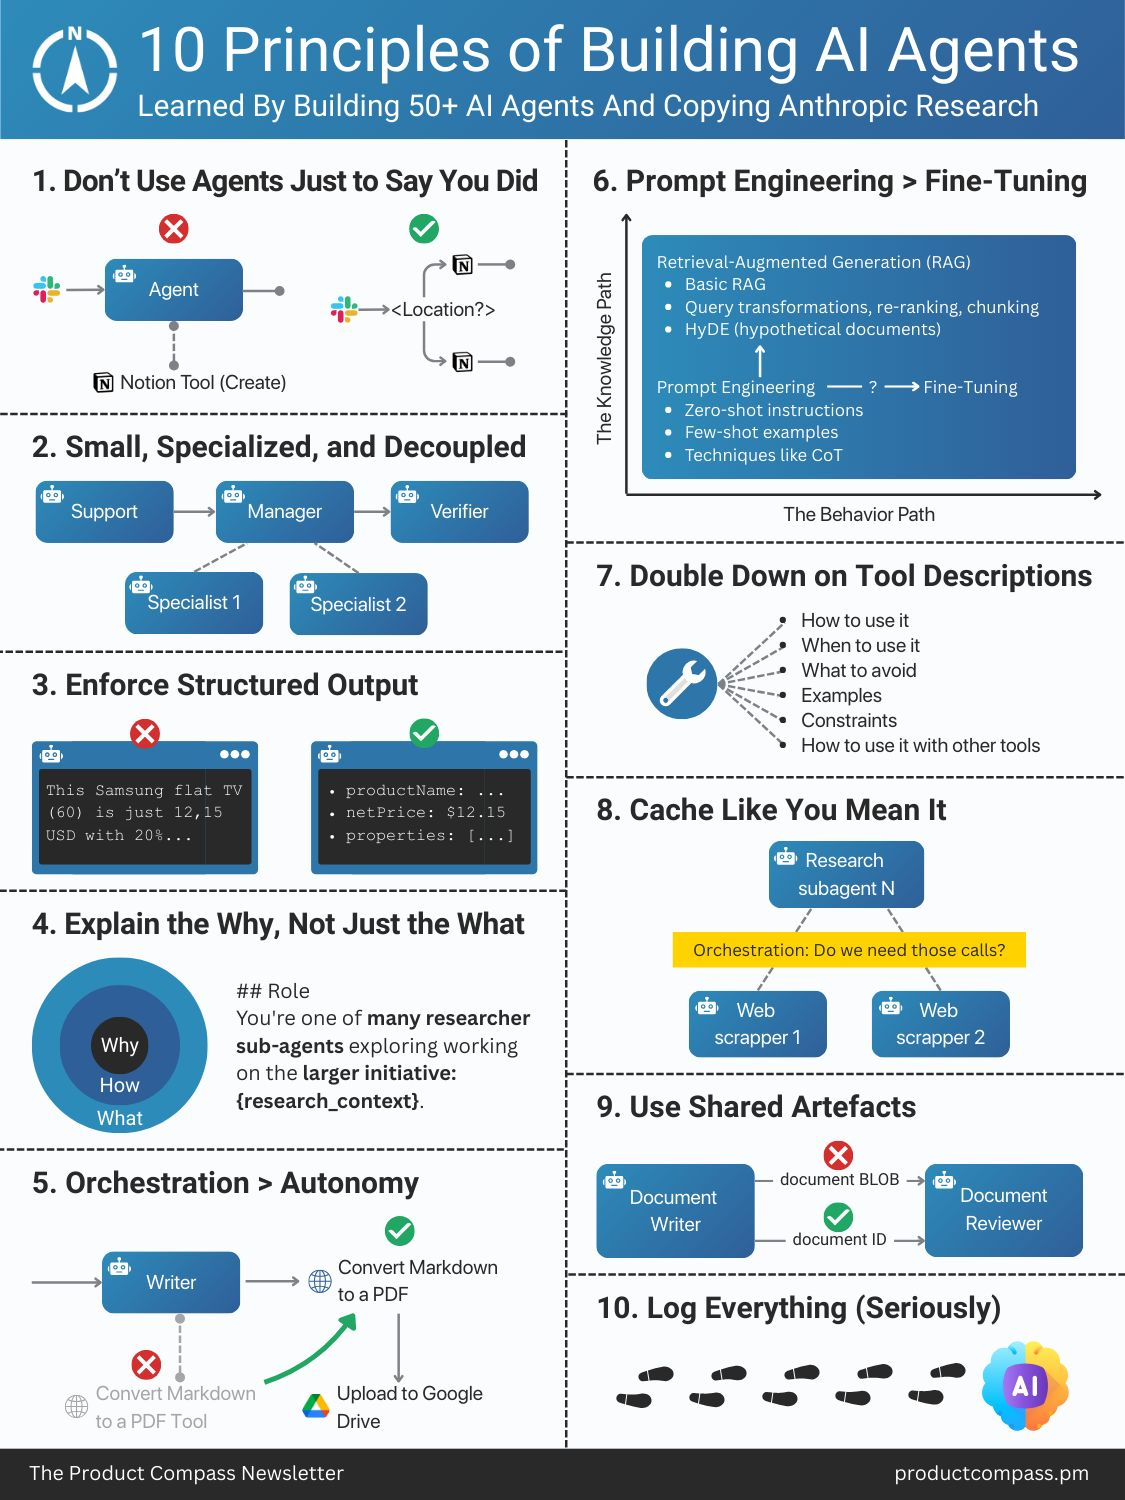
\includegraphics[width=0.6\linewidth,keepaspectratio]{aiagents91}
		
		{\tiny (Ref: Principles of Building AI Agents - Pawel Huryn)}
		\end{center}
\end{frame}

%%%%%%%%%%%%%%%%%%%%%%%%%%%%%%%%%%%%%%%%%%%%%%%%%%%%%%%%%%%%%%%%%%%%%%%%%%%%%%%%%%
\begin{frame}[fragile]\frametitle{Protocols Summary}
		\begin{center}
		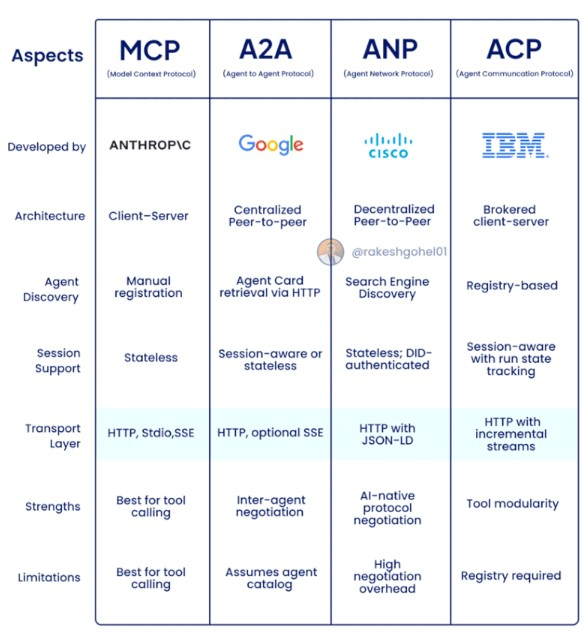
\includegraphics[width=\linewidth,keepaspectratio]{aiagents16}
		\end{center}
		
		{\tiny (Ref: LinkedIn post by Rakesh Gohel)}
\end{frame}
  

%%%%%%%%%%%%%%%%%%%%%%%%%%%%%%%%%%%%%%%%%%%%%%%%%%%%%%%%%%%%%%%%%%%%%%%%%%%%%%%%%%
\begin{frame}[fragile]\frametitle{Are you creative enough?}
		\begin{center}
		\includegraphics[width=\linewidth,keepaspectratio]{autoagent8}
		\end{center}
		
		{\tiny (Ref: Agentic AI Frameworks \& AutoGen - Chi Wang)}
\end{frame}
  

%%%%%%%%%%%%%%%%%%%%%%%%%%%%%%%%%%%%%%%%%%%%%%%%%%%%%%%%%%%
\begin{frame}[fragile]\frametitle{My Sketchnote}
	
	\begin{center}
	\includegraphics[width=0.45\linewidth,keepaspectratio]{AutonomousAIAgents_Sketchnote}
	\end{center}
{\tiny (Ref: Power of Autonomous AI Agents - Yogesh Kulkarni)}
\end{frame}

%%%%%%%%%%%%%%%%%%%%%%%%%%%%%%%%%%%%%%%%%%%%%%%%%%%%%%%%%%%
\begin{frame}[fragile]\frametitle{The Future with AutoGen}
  \begin{itemize}
    \item Transformative era in AI collaboration is on the horizon.
    \item Microsoft's vision for Autonomous AI Agents and AutoGen's capabilities provide a glimpse into the future of AI applications.
    % \item Collaboration, innovation, and democratization are at the core of AutoGen's mission.
    \item Empowers professionals to navigate the complex AI landscape with confidence, agility, and precision.
    % \item The journey has just begun, and the possibilities with AutoGen are endless.
  \end{itemize}
\end{frame}

%%%%%%%%%%%%%%%%%%%%%%%%%%%%%%%%%%%%%%%%%%%%%%%%%%%%%%%%%%%
\begin{frame}[fragile]\frametitle{Towards Artificial General Intelligence (AGI)}
  \begin{itemize}
    \item Research aligns with the belief that achieving human-like general intelligence requires cooperation among agents.
    \item Multi-agent collaboration is a crucial approach, but it may not alone pave the path to artificial general intelligence (AGI).
    \item The journey likely demands additional innovations and breakthroughs.
	\item AutoGen stands out as an enticing platform for exploring possibilities offered by multi-agent systems.
  \end{itemize}
\end{frame}
